\documentclass{article}
\usepackage[utf8]{inputenc}
\usepackage{hyperref}
\usepackage[letterpaper, portrait, margin=1in]{geometry}
\usepackage{enumitem}
\usepackage{amsmath}
\usepackage{booktabs}
\usepackage{graphicx}
\usepackage{float}

\usepackage{hyperref}
\hypersetup{
colorlinks=true,
    linkcolor=black,
    filecolor=black,      
    urlcolor=blue,
    citecolor=black,
}
\usepackage{natbib}

\usepackage{titlesec}
  
\title{Homework 8}
\author{Lin Yang}
\date{\today}
  
\begin{document}
\maketitle  
\section{Stata}
~\\
1. A yearly plot of the recycling rate for NYC and controls. 
\begin{figure}[H]
\centering
\includegraphics[scale = 0.9]{q1.pdf}
	
\end{figure}

~\\
2. By using the TWFE regression, the average treatment effect estimate is -0.0619874 and the standard error is 0.0058239.  


~\\
3. By using synthetic DID, the average treatment effect estimate is -0.06310 and the standard error is  0.03776. The synthetic DID plot is listed below. 
\begin{figure}[H]
\centering
\includegraphics[scale = 0.9]{q3.pdf}
	
\end{figure}


~\\
4. Compared to the year 2001, the average recycling rate decreased by 0.0661686 in year 2002 with standard error of 0.0073971. The event study plot is listed below. 
\begin{figure}[H]
\centering
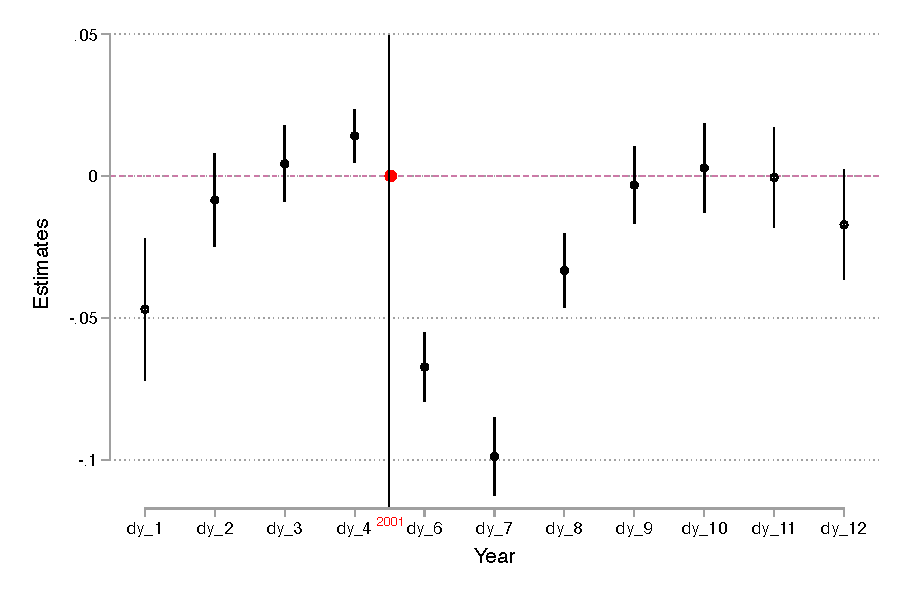
\includegraphics[scale = 0.9]{question4.pdf}	
\end{figure}


~\\
5. (a) The plot of raw outcomes for treated and control groups over time is listed below.
\begin{figure}[H]
\centering
\includegraphics[scale = 0.9]{question5a.pdf}	
\end{figure}
~\\

(b) The plot of raw outcomes for treated group and synthetic group over time is listed below. 
\begin{figure}[H]
\centering
\includegraphics[scale = 0.9]{question5b.pdf}	
\end{figure}

~\\

(c) The plot of estimated synthetic control effects and placebo effects over time is listed below. 
\begin{figure}[H]
\centering
\includegraphics[scale = 0.9]{question5c.pdf	}
\end{figure}



~\\

(d) The plot of final synthetic control estimates over time is listed below. 

\begin{figure}[H]
\centering
\includegraphics[scale = 0.9]{question5d.pdf	}
\end{figure}





\end{document}
